\documentclass[11pt]{article}
\usepackage[margin=1.0in]{geometry}
\usepackage[hidelinks,pdfencoding=auto,psdextra]{hyperref}
\usepackage{amsmath}
\usepackage{graphicx}
% \usepackage[extendedchars]{grffile}
\usepackage{chngpage}
\usepackage{calc}
\usepackage[skip=1pt,font=small]{caption}

\title{Propagation of simulated millicharged particles to the Milliqan detector}

\author{C. Campagnari, B. Marsh (UCSB), F. Golf (UNL)}

\setlength{\parindent}{0em}
\setlength{\parskip}{0.5em}

\begin{document}
\maketitle


\section{Introduction}
In this note we describe the procedure used to propagate simulated millicharged
particles (mCPs) through the CMS environment to the Milliqan detector face. The goals 
of this are to (1) calculate the acceptance of the Milliqan detector (and thus,
when combined with $\sigma\times\mathcal{B}$, the rate of incidence of mCPs),
and (2) generate ``hits'' on the Milliqan detector face  (position and momentum of incoming mCPs)
that can be fed into more sophisticated Geant4 simlations of the detector.

There are four main components to this simulation, listed here and then described in more
detail in the following sections:
\begin{enumerate}
\item Propagation through the CMS magnetic field
\item Multiple scattering while traveling through matter
\item Energy loss while propagating through matter
\item Computation of intersection with Milliqan detector face
\end{enumerate}

All of the code for the propagation is contained in the \href{https://github.com/bjmarsh/MilliqanSim}{\underline{\bf MilliqanSim}} GitHub repository.

\section{Propagation through the CMS magnetic field}
At its core the simulation uses a fourth-order Runge-Kutta integrator to step a charged particle
through a magnetic field. The basic equations of motion are
\begin{equation}\label{eq:dxdt}
\frac{d\vec{x}}{dt} = \vec{v} = \frac{\vec{p}c^2}{E} = \frac{\vec{p}c^2}{\sqrt{(\vec{p}c)^2+(mc^2)^2}}, \\
\end{equation}
\begin{equation}\label{eq:dpdt}
\frac{d(\vec{p}c)}{dt} = qc\;\vec{v}\times\vec{B}.
\end{equation}
If $B$ is in Tesla, $t$ in ns, velocity in m/ns, charge in units of $e$, and $\vec{p}c$ in MeV, the latter becomes
\begin{equation}\label{eq:dpdt_mod}
\frac{d(\vec{p}c)}{dt} = 89.8755\;q\;\vec{v}\times\vec{B}.
\end{equation}

\begin{figure}
\centering
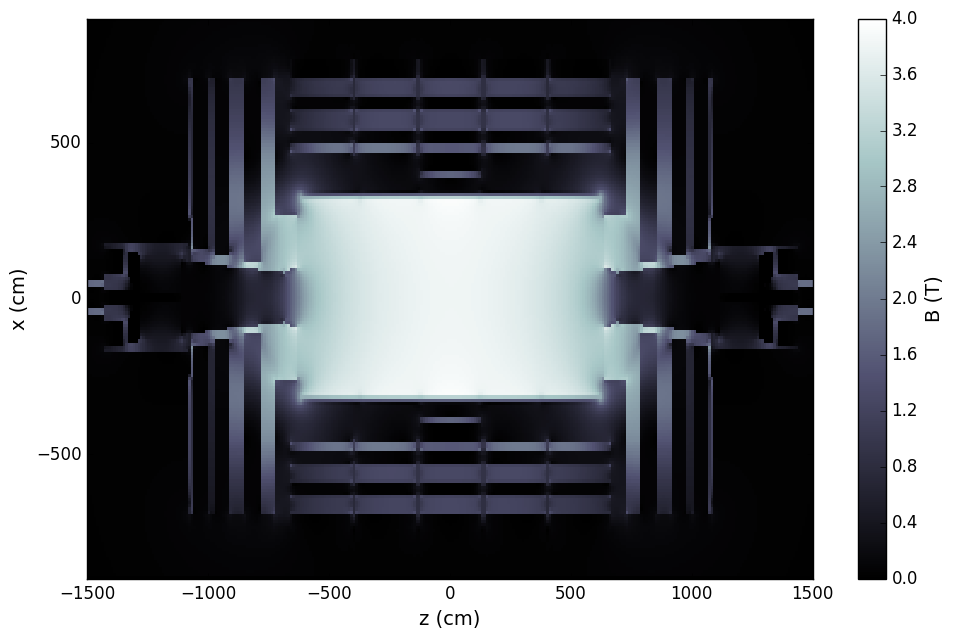
\includegraphics[width=0.7\textwidth]{plots/cms_bfield_coarse.png}
\caption{Magnitdue of the CMS magnetic field, in the $y=0$ plane.}
\label{fig:bfield}
\end{figure}

The magnetic field for CMS has been extracted from CMSSW
in a 3-dimensional cylindrical grid in increments of $\Delta r=10$ cm, $\Delta z=10$ cm, $\Delta\theta=5^\circ$, out to
$r=10$ m and $z=\pm15$ m. A map of the magnitude in the $y=0$ plane is shown in Fig.~\ref{fig:bfield}.
[\emph{Note: we extracted this B-field map from CMSSW, which isn't public. But there are CMS publications (e.g. \cite{CMS_bfield}) that measure
this, so I guess we can plausibly say we got it from those.}]

At each timestep, the magnetic field is determined from ths pre-loaded map and used in the equation of motion (\ref{eq:dpdt_mod}).
The field is interpolated between the two nearest points in $r$ (not $z$ or $\theta$, since for the region of interest the field
is essentially flat over these variables).

For now, the simulation uses a timestep of $dt=0.1$ ns, corresponding to a distance $dx\approx3$ cm for a particle traveling near
the speed of light. This can probably be increased without meaningfully changing the results, in order to speed up computation time.

\section{Material model of CMS and surroundings}
In order to simulate the interactions of particles with matter, a model of CMS has been extracted from a public ROOT model \cite{ROOT_cms}.
At each point in space, it is possible to get the material as well as it's properties. A plot of $\rho Z/A$ as a function of radius is
shown in Fig. \ref{fig:cmsdensity}. This is used to construct a simplified model of CMS for the purposes of particle propagation.
For simplicity, all material lengths are converted into ``equivalent distance of iron'' by scaling by the $\rho Z/A$ ratio. Then concentric
cylinders of iron are placed between the following radii:
\begin{itemize}
\item $1.80 \leq r < 2.80$ m (tracker + HCAL)
\item $3.15 \leq r < 3.50$ m (magnet)
\item $3.85 \leq r < 4.05$ m (return yoke 1)
\item $4.60 \leq r < 4.95$ m (return yoke 2)
\item $5.35 \leq r < 5.95$ m (return yoke 3)
\item $6.35 \leq r < 7.15$ m (return yoke 4)
\end{itemize}

\begin{figure}
\centering
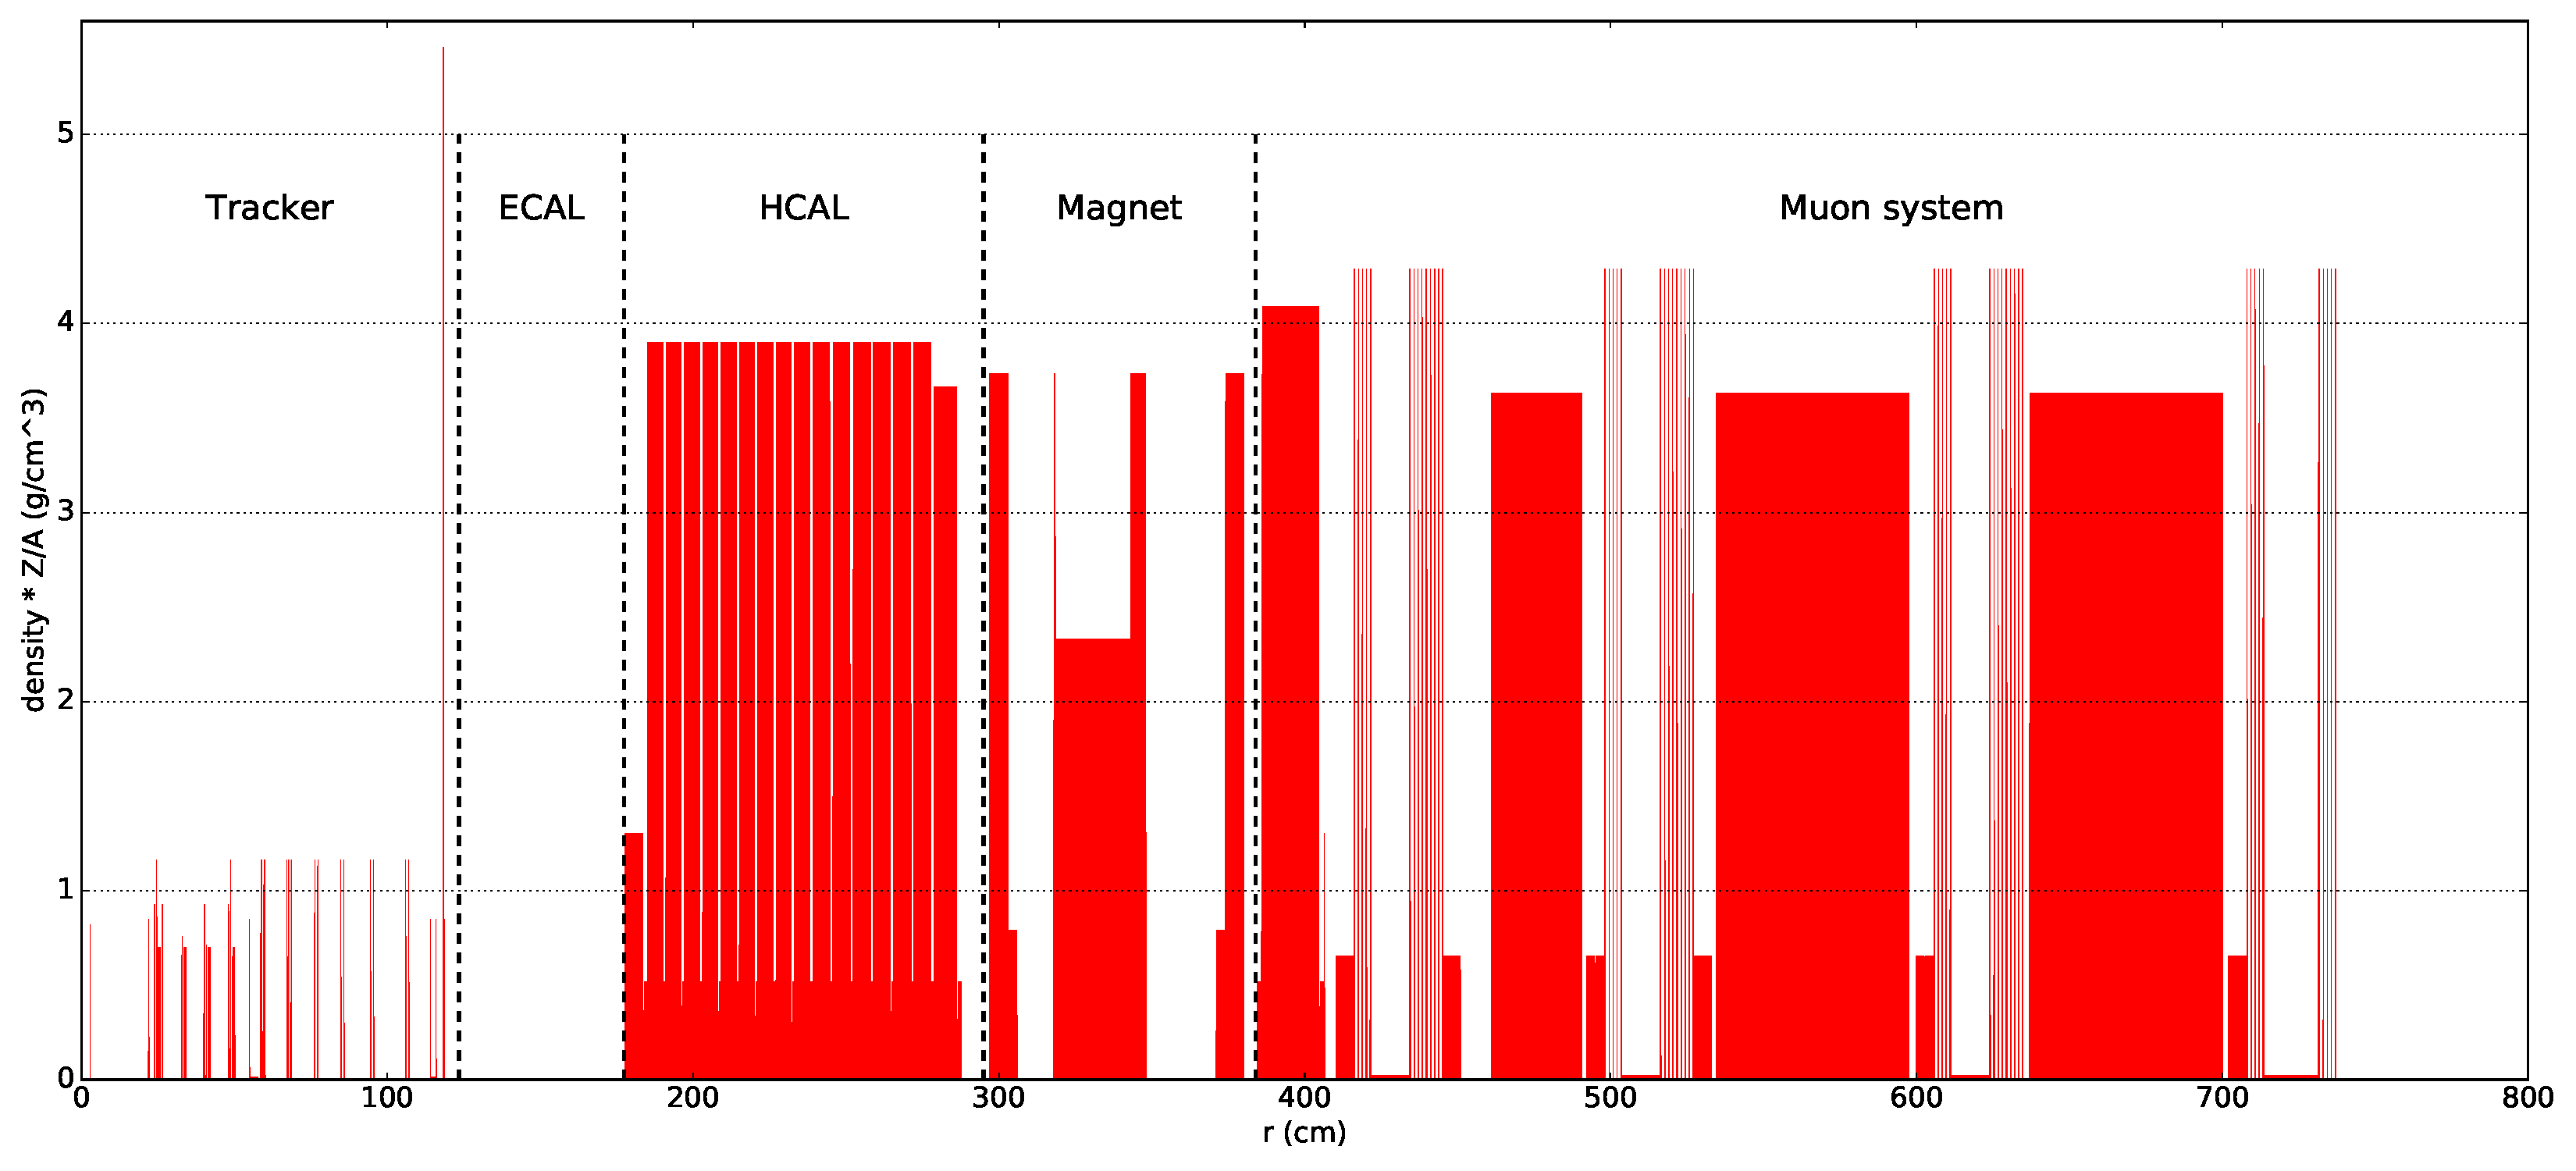
\includegraphics[width=0.99\textwidth]{plots/cms_density_map.pdf}
\caption{A map of material $\rho Z/A$ as a function of radius for CMS, as extracted from a public ROOT model of CMS \cite{ROOT_cms}.
Note that ECAL is missing, so we add 25 cm of PbWO$_4$. between radii of 1.25 and 1.50 m.}
\label{fig:cmsdensity}
\end{figure}

The total amound of iron is 3.30 m. In addition, 25 cm of PbWO$_4$ is placed between $1.25 < r < 1.50$ m to account for the ECAL crystals.

Rock is placed between $15.8 < R < 32.8$ m to account for the 17 meters of rock between the IP and Milliqan. All space not filled by
iron, PbWO$_4$, or rock by the above rules is set to air.

\section{Multiple scattering through matter}
Two methods of implementing multiple scattering have been studied. The first assumes purely small-angle gaussian scattering, and is described
in the PDG chapter on the passage of particles through matter \cite{PDG_matter}. The second is a bit more complicated but more realistically
simulates the larger, non-gaussian tails present in true multiple scattering. It is outlined in a paper by Kuhn and Dodge \cite{kuhn_msc}.
The prediction using the Kuhn algorithm agrees better with measured muon rates at Milliqan (the predicted slab rate is 10\% lower
compared to the prediction using the PDG algorithm), but uncertainties are relatively large
so it is difficult to say definitively that it is more accurate.
The following sections briefly summarize the implementations of both of these algorithms.

\subsection{``PDG algorithm'' for multiple scattering}
\label{sec:pdg_msc}

The simpler implementation of multiple scattering is taken from the PDG chapter on the passage of particles through matter \cite{PDG_matter}.
This assumes a small-angle gaussian scattering, and does not take into account non-gaussian tails from rare hard scatters. 
The algorithm consists of picking two random scattering angles independently in orthogonal directions, as well as correlated transverse displacements.

The RMS of the scattering angle distribution is given by
\begin{equation}\label{eq:thrms}
\theta_0 = \frac{13.6~\text{MeV}}{\beta cp}\;z\;\sqrt{\frac{x}{X_0}}\left[1 + 0.088\log_{10}\left(\frac{xz^2}{X_0\beta^2}\right) \right],
\end{equation}
where $p$, $\beta c$, and $z$ are the momentum, velocity, and charge number of the incident particle, $x$ is the distance traversed, and 
$X_0$ is the radiation length of the material.

In addition to an angular deflection $\theta_\text{plane}$, there is a correlated transverse deviation $y_\text{plane}$ (see Fig. \ref{fig:mscangles}). The correlation coefficent
turns out to be $\sqrt{3}/2\approx0.87$, and it is sufficient to generate two independent gaussian random variables $z_1,z_2$ and compute
\begin{equation}\label{eq:msc}
y_\text{plane} = z_1\;x\;\theta_0/\sqrt{12} + z_2\;x\;\theta_0/2
\end{equation}
\[
\theta_\text{plane} = z_2\;\theta_0.
\]

This is done independently in both directions orthogonal to the direction of travel.

\begin{figure}
\centering
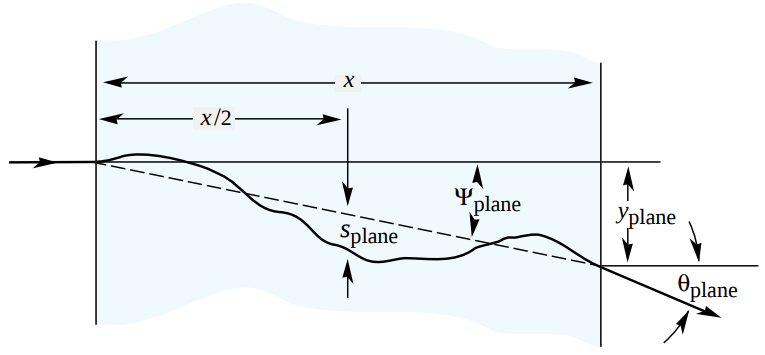
\includegraphics[width=0.7\textwidth]{plots/pdg_msc_diagram.png}
\caption{Diagram showing the defined $\theta_\text{plane}$ and $y_\text{plane}$ variables used to describe the PDG algorithm for multiple scattering.}
\label{fig:mscangles}
\end{figure}

\subsection{``Kuhn algorithm'' for multiple scattering}
\label{sec:kuhn_msc}

The second algorithm more accurately models the larger, non-gaussian tails of the scattering angle distribution at each timestep. It essentially
piecewise-joins a gaussian core with non-gaussian tails modeled by the Rutherford scattering law. Details of the derivation are given 
in \cite{kuhn_msc}. Here we describe the technical implementation.

First, constants are defined:
\begin{equation}\label{eq:kuhn_chi}
\chi_c^2 = 0.1569\,\frac{z^2Z(Z+1)}{(pc)^2\beta^2}\frac{\rho\Delta s}{A}
\end{equation}
and
\begin{equation}\label{eq:kuhn_B}
B_0-\log(B_0) = \log\left(\frac{6700z^2Z^{1/3}(Z+1)\rho\Delta s/A}{\beta^2+(1.77\times10^{-4})z^2Z(Z+1)}\right),
\end{equation}
where $z$ is the charge of the projectile (in units of $e$), 
Z and A are the effective atomic number and atomic weight of the target material, respectively, 
$\beta=v/c$ is the velocity of the projectile, $pc$ is its momentum (in MeV), and
$\rho$ is the density of the target material in g/cm$^3$. 
These are taken from the original analytical formulation of multiple scattering by Moli\`ere. The replacement
of $Z^2$ by $Z(Z+1)$ and $Z^{4/3}$ by $Z^{1/3}(Z+1)$ are due to the correction for highly relativistic particles
derived by Bethe. The constant $B_0$ is defined as a part of a transcendental equation, so it is solved for
numerically using the Newton-Raphson method. For the following, we use a modified $B=B_0+1$
rather than $B_0$ straight from Eq. \ref{eq:kuhn_B}. 
This was found by Kuhn to fix an empirically too-narrow final distribution.

The core of the scattering angle distribution is described by a gaussian of width
\begin{equation}\label{eq:kuhn_th1e}
\theta_{1/e} = \chi_c\sqrt{B-1.25}.
\end{equation}
The cumulative distribution function (i.e. the probability for the scattering angle to be between 0 and $\theta$) is then given by
\begin{equation}
\begin{split}
P(\theta)=(1-0.827&/B)\left\{1-\exp\left[-\left(\frac{\theta}{\theta_{1/e}}\right)^2\right]\right\} \\
&+\Theta(\theta-\sqrt{2}\theta_{1/e})\frac{\chi_c^2}{4}\left(\frac{1}{\sin^2(\theta_{1/e}/\sqrt{2})}-\frac{1}{\sin^2(\theta/2)}\right).
\end{split}
\end{equation}

This is not quite normalized correctly, as $P(\pi)$ is slightly below 1. So we compute
\begin{equation}\label{eq:kuhn_ppi}
P(\pi) = 1-0.827\frac{1}{B}+\frac{\chi_c^2}{4}\left(\frac{1}{\sin^2(\theta_{1/e}/\sqrt{2})} - 1\right).
\end{equation}

Then the actual algorithm is as follows: 
\begin{enumerate}
\item Compute $\chi_c$ from Eq.~\ref{eq:kuhn_chi}, solve Eq.~\ref{eq:kuhn_B} for $B_0$ and add 1 to get $B$,
and plug these into Eqs.~\ref{eq:kuhn_th1e} and \ref{eq:kuhn_ppi} to get $\theta_{1/e}$ and $P(\pi)$.
\item Generate a random number $R$ in $[0,P(\pi)]$.
\item If $R\geq1-0.827/B$, then
\[
R' = R - 1 + 0.827/B
\]
\begin{equation}
\theta = 2\sin^{-1}\left(\frac{\chi_c\sin(\theta_{1/e}/\sqrt{2})}{\sqrt{\chi_c^2-4R'\sin^2(\theta_{1/e}/\sqrt{2})}}\right).
\end{equation}
\item Otherwise, if $R<1-0.827/B$, then
\begin{equation}
\theta = \theta_{1/e}\left[\log\left(\frac{1-0.827/B}{1-0.827/B-R}\right)\right]^{1/2}.
\end{equation}
\item Generate a random $\phi$ in $[0,2\pi]$. Then the particle's new direction of propagation is given by $(\theta,\phi)$ 
in spherical coordinates centered on its original direction of propagation.
\end{enumerate}

The Kuhn algorithm does not provide for any transverse displacement on top of the angular deflection at each timestep.
However, the paper shows that the final spatial distribution of a particle is well described by this algorithm
using only angular deflections at each timestep.

\subsection{Comparison of algorithms}
Figure \ref{fig:msccomp} (left) shows a comparison of the scattering angle for a 16 GeV muon traversing 3 cm of iron,
using either the PDG or Kuhn multiple scattering algorithms. The small-angle gaussian cores agree well, while the 
Kuhn algorithm has a substantially larger tail.

Figure \ref{fig:msccomp} (right) shows a comparison of projected angular distributions for muons incident on the Milliqan detector face,
using either the PDG or Kuhn algorithms. The width of the central gaussian core does not change much
($1.07^\circ$ vs. $1.14^\circ$). However, there is a small but noticable shift in the Kuhn algorithm to a smaller core and
larger tails, as might be expected. The overall fraction of events in the fitted gaussian core goes from 74\% o 70\%,
but the decrease in the central-most region (less than $\sim$1$^\circ$) most relevant for through-going particles
is closer to 10\%. This corresponds well with an observed decrease in predicted four-slab muon rate of
about 10\% when switching to the Kuhn algorithm.


\begin{figure}
\centering
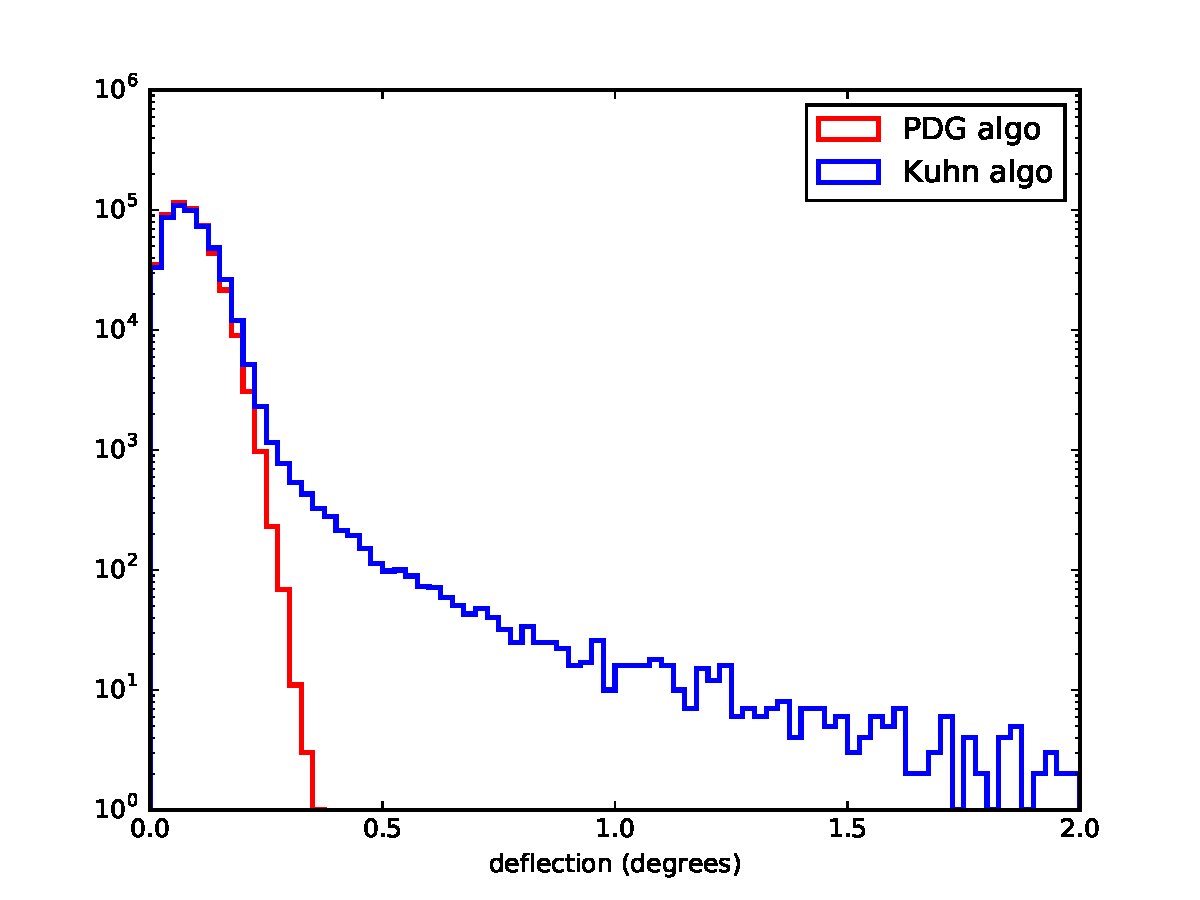
\includegraphics[width=0.47\textwidth]{plots/pdg_kuhn_single_comp.pdf}
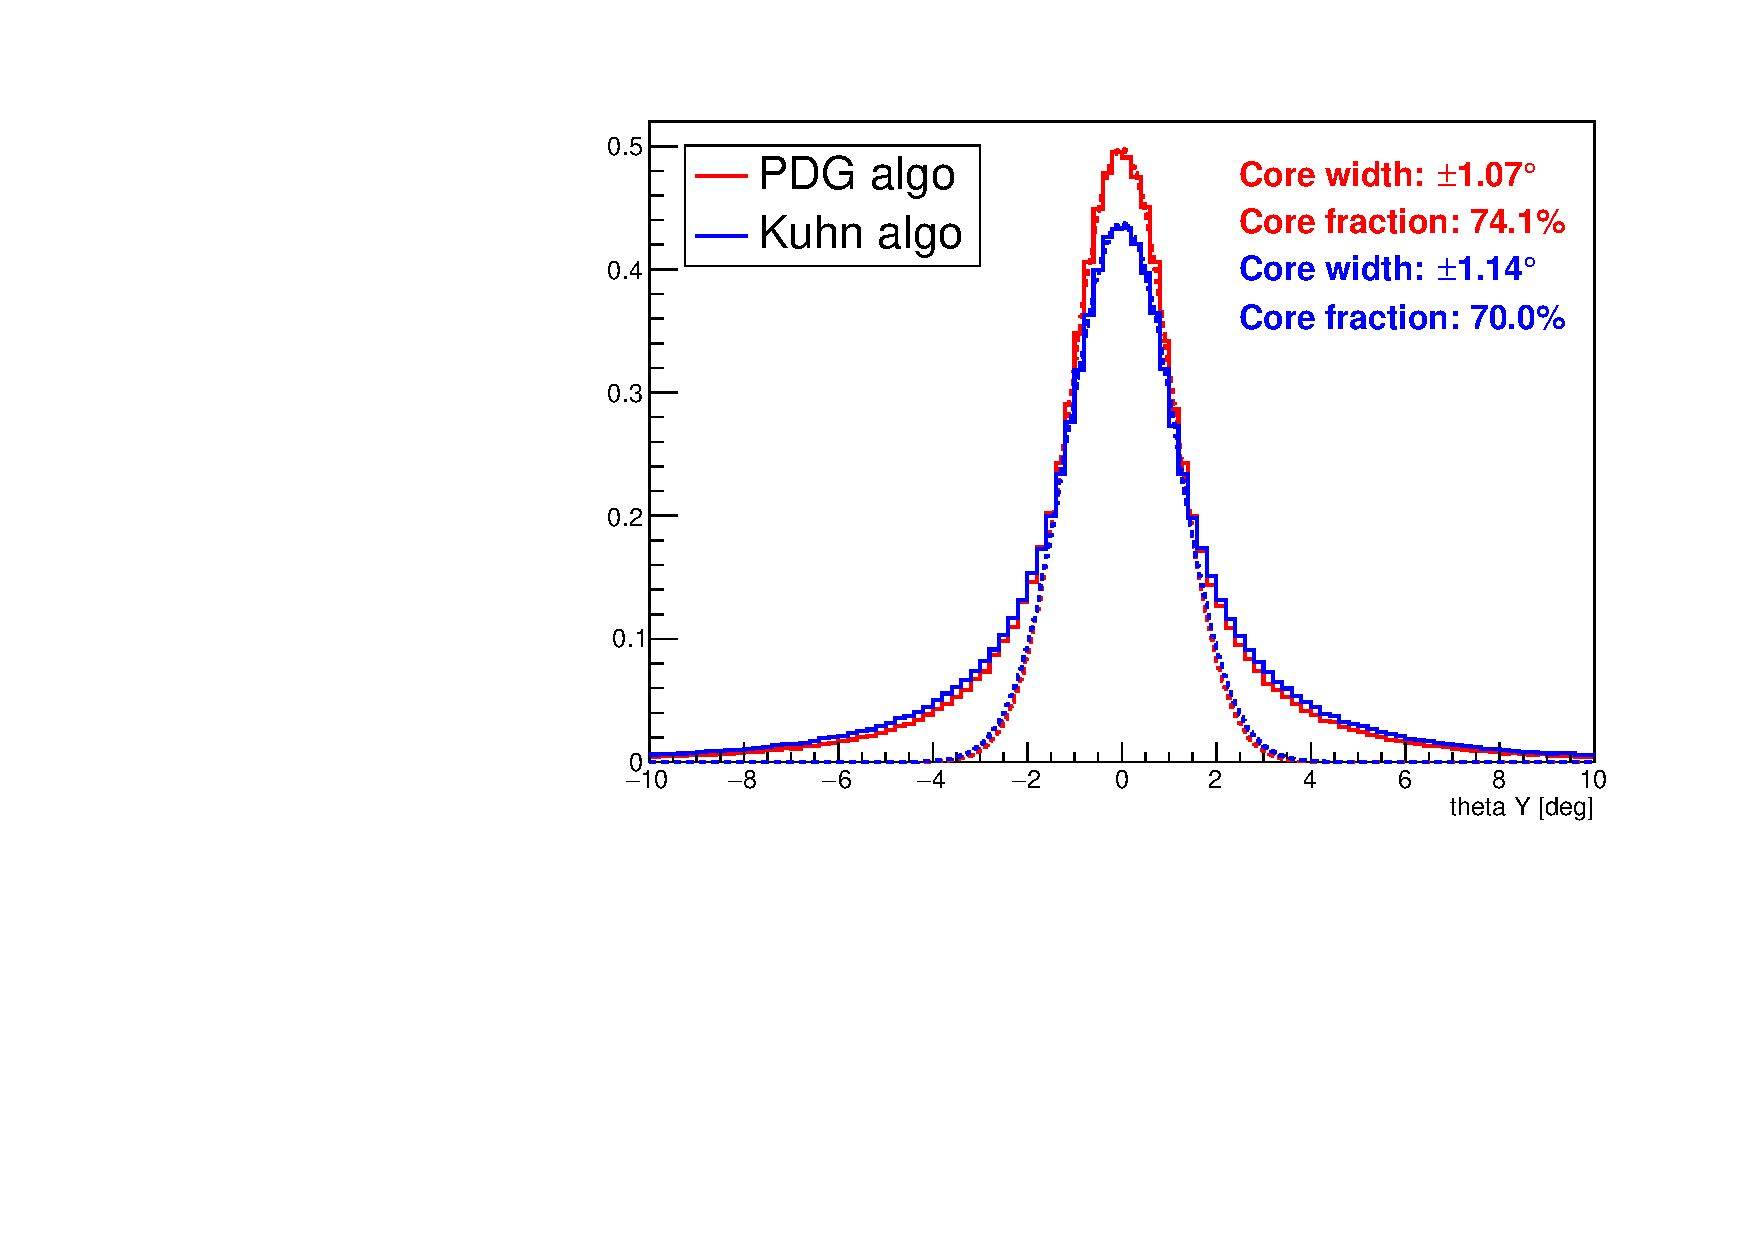
\includegraphics[width=0.52\textwidth]{plots/pdg_kuhn_final_comp.pdf}
\caption{(left) The scattering angle distribution of a 16 GeV muon through 3 cm of iron, as simulated with the PDG algorithm (red) or the Kuhn algorithm (blue). 
Note the much larger high-angle tail when using the Kuhn algorithm.
(right) The distribution of incidence angles (projected into the horizontal plane) of muons on the Milliqan detector face for each algorithm.
Dotted lines are gaussian fits to the cores of the distributions. The Kuhn algorithm slightly
enlarges the tails of the distribution, and reduces the probability near $\theta=0^\circ$ by $\sim$10\%.}
\label{fig:msccomp}
\end{figure}

\section{Energy loss}
In addition to multiple scattering, particles lose energy as they propagate through matter. This is implemented using the 
Bethe formula
\begin{equation}\label{eq:dedx}
\left\langle-\frac{dE}{dx}\right\rangle = Kz^2\frac{Z}{A}\frac{1}{\beta^2}\left[\frac{1}{2}\log\frac{2m_ec^2\beta^2\gamma^2W_\text{max}}{I^2} - \beta^2 - \frac{\delta(\beta\gamma)}{2} \right].
\end{equation}

For definitions of all terms and parameters, see \cite{PDG_matter}. All material constants are taken from \cite{PDG_properties}.
Note that energy loss is a stochastic process, and at each timestep the actual energy loss follows a highly skewed Landau distribution.
However, the amount of material traversed in this application is quite large, so it should be sufficient to use the mean value
at each timestep. At any rate, a systematic is assessed on the interaction with matter that should cover for any inaccuracies
in the modeling of energy loss.


\section{Putting it all together}
At each timestep, the following steps are taken:
\begin{enumerate}
\item Evaluate $d\vec{x}/dt$ and $d\vec{p}/dt$ using using the current position/momentum $\vec{x}_i/\vec{p}_i$ inserted into Eqs. \ref{eq:dxdt} and \ref{eq:dpdt_mod} (actually,
evaluate four times as per the Runge-Kutta method). Use the Runge-Kutta method to compute $\Delta\vec{x}_{\text{B},i}$ and $\Delta\vec{p}_{\text{B},i}$ for the timestep.
\item Look up the material at $\vec{x}_i$, and use this to perform multiple scattering. 
This is done with either the PDG (Sec.~\ref{sec:pdg_msc}) or Kuhn (Sec.~\ref{sec:kuhn_msc}) algorithms.
Use the computed angular deflection and transverse displacement (PDG only) to get $\Delta\vec{x}_{\text{MS},i}$ and $\Delta\vec{p}_{\text{MS},i}$ due to multiple scattering.
\item Use material constants to evaluate $dE/dx$ with Eq. \ref{eq:dedx}. Multiply by $\delta x=v\delta t$ to get $\delta E$, and use this to compute $\Delta\vec{p}_{\text{EL},i}$.
\item The total changes in position and momentum for the timestep are then $\Delta\vec{x}_i = \Delta\vec{x}_{\text{B},i}+\Delta\vec{x}_{\text{MS},i}$ and
$\Delta\vec{p}_i = \Delta\vec{p}_{\text{B},i}+\Delta\vec{p}_{\text{MS},i}+\Delta\vec{p}_{\text{EL},i}$.
\end{enumerate}

This is done for $N_\text{steps}$ timesteps (or until a specified distance cutoff is reached). At the end we get an array of $(t,x,y,z,p_x,p_y,p_z)$ values at each timestep.

\section{Intersection with the Milliqan Detector}
To facilitate acceptance and rate calculations, tools have been added to the simulation to compute intersections with
various detector models.

For simple applications, one can find intersections with an external plane and retrieve the position and momentum
at the intersection. This is useful for gathering four-vectors to feed into an external simulation of the detector.

The ability to construct a ``Milliqan-type'' detector with arbitrary numbers of bars has also been added.
The entry/exit points for each individual bar can be computed, so that for each trajectory one can determine
the number of bars hit, whether those bars are in a line, the length of the path traversed within the bar, etc.
An example of two mCPs hitting the Milliqan demonstrator is shown in Fig. \ref{fig:traj_vis}.

\begin{figure}
\centering
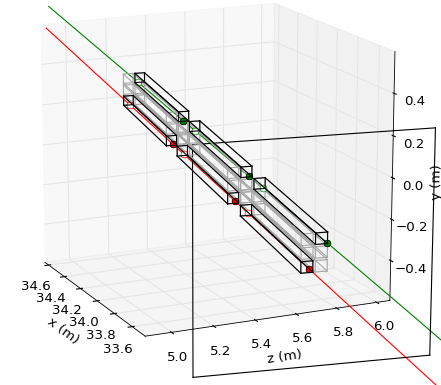
\includegraphics[width=0.7\textwidth]{plots/traj_vis.png}
\caption{Visualization of two mCP trajectories passing through the Milliqan demonstrator.}
\label{fig:traj_vis}
\end{figure}


\begin{thebibliography}{1}

\bibitem{CMS_bfield} CMS Collaboration, ``Precise mapping of the magnetic field in the CMS barrel yoke using cosmic rays''.
\emph{Journal of Instrumentation} {\bf 5} (2010) no. 3, T03021. \href{https://doi.org/10.1088\%2F1748-0221\%2F5\%2F03\%2Ft03021}{doi:10.1088/1748-0221/5/03/t03021}.

\bibitem{ROOT_cms} ROOT, \href{https://root.cern/files/cms.root}{https://root.cern/files/cms.root}

\bibitem{PDG_matter}  PDG, chapter 33. ``Passage of particles through matter''.
[\href{http://pdg.lbl.gov/2019/reviews/rpp2018-rev-passage-particles-matter.pdf}{link}]

\bibitem{PDG_properties}  PDG, ``Atomic and Nuclear Properties of Materials''.
[\href{http://pdg.lbl.gov/2019/AtomicNuclearProperties/index.html}{link}]

\bibitem{kuhn_msc} Kuhn, S. and Dodge, G. ``A fast algorithm for Monte Carlo simulations of multiple Coulomb scattering''.
\emph{Nucl. Instrum. Methods Phys.} {\bf A322} (1992), iss. 2, 88. \href{https://doi.org/10.1016/0168-9002(92)90361-7}{doi:10.1016/0168-9002(92)90361-7}.

\end{thebibliography}
  
\end{document}
